\subsection{Data reduction analysis} 
\label{sec:dedup_ratio}

\paragraph{Layer sharing}

In its simplest implementation Docker would not support layer sharing.
%
Instead, every image would be a single flat archive.
%
In fact, some existing containerization frameworks
~\cite{singularity}~\cite{openvz} 
%
\VT{cite singularity and openvz}
%
\NZ{addressed}
%
\VT{No, not addressed, citation for singularity is still missing}
%
use flat images.
%
Our estimates show that without layer sharing Docker Hub dataset would grow
from 47TB to 85TB, implying \textbf{1.8$\times$} deduplication ratio provided
by the layer sharing technique.
 
We further computed for each layer, how many times it is referenced by images.
%
Figure~\ref{fig:ref_count} shows that around 90\% of layers are referenced by
only a single image, additional 5\% are referenced by 2 images, and less than
1\% of the layers are shared by more than 25 images.
%
Interestingly, there is one layer that is referenced by 184,171 images.  Our
analysis revealed that this is an empty layer. 
%
In addition, we found 7 layers that are referenced by 29,200 - 33,413 images.
They are mainly related to ubuntu 14.04.2, dpkg, apt, and cowsay. 
\NZ{Some layer tarfiles are not easy to describe. AND. these above layers are not 
	referred by official Ubuntu latest. Find an interesting thing: image name already
	tells what software packages it contains.} 
%
\VT{Explain the reason for empty layer.}
%
\VT{I feel we might need to talk about 2 more "most referenced" layers.}
\NZ{addressed}
%
\VT{Use \% instead of probability in all Figures (both  \# and labels).
We use \% in the text, so we MUST do it.}

\begin{figure}[t]
	\centering
		\begin{minipage}{0.2\textwidth}
			\centering
			\includegraphics[width=1\textwidth]{graphs/shared-cnt-cdf.pdf}
			\caption{CDF of layer reference count.}
			\label{fig:ref_count}
		\end{minipage}
	\begin{minipage}{0.22\textwidth}
		\centering
		\includegraphics[width=1\textwidth]{graphs/layer-size-cdf.pdf}
		\caption{CDF of compress. and uncompress. layer size.}
		\label{fig:layer-size-cdf}
	\end{minipage}%
\end{figure}
%%		\vcomment{Figures \ref{fig:layer-size-cdf} and \ref{fig:compress-ratio}
%have different sizes, looks not neat, please fix.}
%\begin{figure}
%	\centering
%	\includegraphics[width=0.21\textwidth]{graphs/shared-cnt-cdf.pdf}
%	\caption{CDF of layer reference count.
%	}
%	\label{fig:ref_count}
%\end{figure}
%
%+-----------------------------------------------------------------------+----------------+
%|layer_id                                                               |shared_image_cnt|
%+-----------------------------------------------------------------------+----------------+
%|sha256:a3ed95caeb02ffe68cdd9fd84406680ae93d633cb16422d00e8a7c22955b46d4|184171          | empty
%|sha256:e190868d63f8f8b85b026e53b5724c3c2a4548e1d642953442559cfa5f79b2c9|33413           | ubuntu 14.04.2 LTS. 
%|sha256:909cd34c6fd77d398af1d93e9d4f7f76104903f237be3d4db7b345a19631f291|33323           | dpkg
%|sha256:0b9bfabab7c119abe303f22a146ff78be4ab0abdc798b0a0e97e94e80238a7e8|33295           | apt
%|sha256:8eed3712d2cfd8c37b19d324452ba9cdb445933c04c9175c4e945b0d7241f1e3|31517           | cowsay
%|sha256:c57b6bcc83e3e88fb3748ea3f0cb13d77c4e2ffa7b9a8ded3d636f17d2d83759|31503           | cowsay 3.03 installasion package
%|sha256:8978f6879e2f86eb7a063e70f7d89feecde9950c40fc68f1f53d00b3c8ce9b52|31179           | same cowsay but different git info
%|sha256:00bf65475aba8f1077fa9629f088a5f531d645faeccb6acd7a8626c7d896a4c4|29200           | (looks like linux distribution)
%|sha256:386a066cd84a33a04d560c42bef66d1dd64ebfc76de78550e5fd0f8d57778bca|6103            |
%|sha256:3690ec4760f95690944da86dc4496148a63d85c9e3100669a318110092f6862f|4678            |
%|sha256:5c90d4a2d1a8dfffd05ff2dd659923f0ca2d843b5e45d030e17abbcd06a11b5b|4635            |
%|sha256:6d827a3ef358f4fa21ef8251f95492e667da826653fd43641cef5a877dc03a70|4496            |
%|sha256:627beaf3eaaff1c0bc3311d60fb933c17ad04fe377e1043d9593646d8ae3bfe1|4025            |
%|sha256:e110a4a1794126ef308a49f2d65785af2f25538f06700721aad8283b81fdfa58|4001            |
%|sha256:357ea8c3d80bc25792e010facfc98aee5972ebc47e290eb0d5aea3671a901cab|3952            |
%|sha256:6a5a5368e0c2d3e5909184fa28ddfd56072e7ff3ee9a945876f7eee5896ef5bb|3927            |
%|sha256:75ea8418708338e40dce9179cfe97fd116831f1601be50fef48ea6011653c986|3895            |
%|sha256:75a822cd7888e394c49828b951061402d31745f596b1f502758570f2d0ee79e2|3793            |
%|sha256:f94adccdbb9cec09b3e64ec31aab2b07cbc020fe8f9151418ca6b7ede22273c0|3717            |
%|sha256:693502eb7dfbc6b94964ae66ebc72d3e32facd981c72995b09794f1e87bac184|3701            |
%+-----------------------------------------------------------------------+----------------+

\paragraph{Compression}
%
Figure~\ref{fig:layer-size-cdf} presents compressed and uncompressed layer size
distributions.
%
We find that 50\% of the layers are less than 1MB and 90\% of the layers are
less than 64MB in compressed format.
%
If uncompressed, 50\% of the layers are smaller than 2 MB and 90\% of the
layers are smaller than 170MB.
%
Moreover, the total compressed layer dataset grows from 47~TB to 167~TB after decompression, resulting in \textbf{3.6$\times$} compression ratio.

\paragraph{File-level deduplication}
%
Next, we calculate deduplication ratio in terms of file count and capacity for
the complete uncompressed dataset.
%
After removing redundant files, there are only 3.17\% of files left that occupy
23.92~TB, resulting in deduplication ratios of \textbf{31.55$\times$} and
\textbf{6.99$\times$} in terms of file count and capacity, respectively.
%
\begin{figure} \centering
	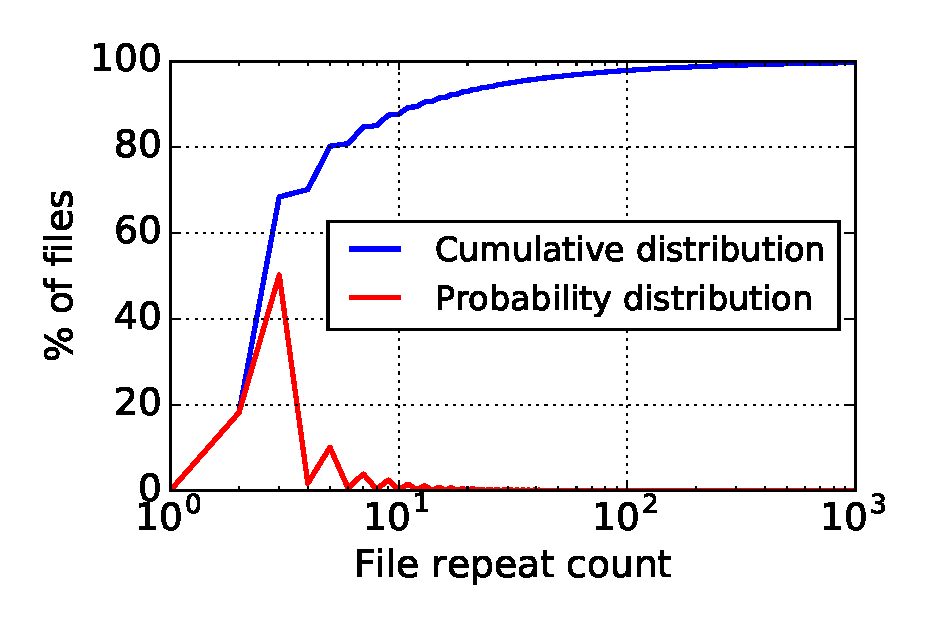
\includegraphics[width=0.45\textwidth]{graphs/File_repeat_count.eps}
	\caption{File repeat count distribution.
	%
	\VT{No need for Y2}
	%
	\VT{Still need to use \% on the axis}
	%
	} \label{fig:file-repeat-cnt}
\end{figure}

%
We further analyzed the repeat count for every file.
%
Figure~\ref{fig:file-repeat-cnt} shows the distributions of file repeat count.  
%
We see that over 99.42\% of files have more than one copy.
%
Around 50\% of files have exactly 4 copies and 90\% of files have 10 or less
copies. 
%
The file that has the maximum repeat count 53,654,306---is an empty file.
%
\VT{Do we know anything about those empty files}.
%

%
\VT{I believe we need to talk about over frequent files. Maybe in the text
section.}.
